\documentclass[12pt,oneside,a4paper,english]{article}
\usepackage[T1]{fontenc}
\usepackage[latin2]{inputenc}
\usepackage[margin=2.25cm,headheight=26pt,includeheadfoot]{geometry}
\usepackage[english]{babel}
\usepackage{color}
\usepackage{titlesec}
\usepackage{titling}
\usepackage[framed, numbered]{matlab-prettifier}
\usepackage{changepage}
\usepackage{amsmath}
\usepackage{hyperref}
\usepackage{enumitem}
\usepackage{graphicx}
\usepackage{fancyhdr}
\usepackage{lastpage}
\usepackage{caption}
\captionsetup[figure]{font=small}
\usepackage{tocloft}
\usepackage{setspace}
\usepackage{multirow}
\usepackage{titling}
\usepackage{float}
\usepackage{comment}
\usepackage{booktabs}
\usepackage{indentfirst}
\usepackage{lscape}
\usepackage{booktabs,caption}
\usepackage[flushleft]{threeparttable}
\usepackage[english]{nomencl}
\usepackage{xcolor}
\usepackage{lipsum}
\usepackage{amsfonts}
\usepackage{array}
\usepackage{hyperref}



\hypersetup{
    colorlinks=true,
    linkcolor=blue,
    filecolor=magenta,      
    urlcolor=cyan,
    pdftitle={Sound Scene Classifier for Hearing Aids},
    pdfpagemode=FullScreen,
    }
    
\urlstyle{same}

% for the first solution
\usepackage{mathtools}
\newcommand{\equalexpl}[1]{%
  \underset{\substack{\uparrow\\\mathrlap{\text{\hspace{-1em}#1}}}}{=}}


% --- set footer and header ---
\pagestyle{fancy}
\fancyhf{}

\usepackage{listings}

\usepackage{xcolor}

%New colors defined below
\definecolor{codegreen}{rgb}{0,0.6,0}
\definecolor{codegray}{rgb}{0.5,0.5,0.5}
\definecolor{codepurple}{rgb}{0.58,0,0.82}
\definecolor{backcolour}{rgb}{0.95,0.95,0.92}

%Code listing style named "mystyle"
\lstdefinestyle{mystyle}{
  backgroundcolor=\color{backcolour}, commentstyle=\color{codegreen},
  keywordstyle=\color{magenta},
  numberstyle=\tiny\color{codegray},
  stringstyle=\color{codepurple},
  basicstyle=\ttfamily\footnotesize,
  breakatwhitespace=false,         
  breaklines=true,                 
  captionpos=b,                    
  keepspaces=true,                 
  numbers=left,                    
  numbersep=5pt,                  
  showspaces=false,                
  showstringspaces=false,
  showtabs=false,                  
  tabsize=2
}

%"mystyle" code listing set
\lstset{style=mystyle}

\setlength{\parindent}{2em}
\title{} % to reference as \title, dont use \maketitle
\makeatletter\let\Title\@title\makeatother

\lstset{language=Matlab,
style=Matlab-editor,
basicstyle=\normalsize\mlttfamily,
numbers=left,
numberstyle={\scriptsize\color{black}},			% size of the numbers
numbersep=0.5cm											
}

\newlist{steps}{enumerate}{1}
\setlist[steps, 1]{leftmargin=1.5cm,label = Step \arabic*:}
\renewcommand{\headrulewidth}{1pt}
\renewcommand{\footrulewidth}{1pt}

%\lhead{\Title}
\rhead{\nouppercase{\rightmark}}
\lhead{\Title}
% \rfoot{\includegraphics[height=1.25cm]{root/logo.pdf}} % right header logo
\setlength\headheight{16pt}
\setlength{\footskip}{50pt}
\lhead{\Title} %rightH title
\cfoot{\thepage}
\setlength\parindent{0pt}

% --- End of page settings ---


\begin{document}

\pagenumbering{roman} 

\begin{titlepage}
\begin{center}
\vspace{0cm}
%\textsc{ Danmarks Tekniske Universitet}\\[1.5cm]
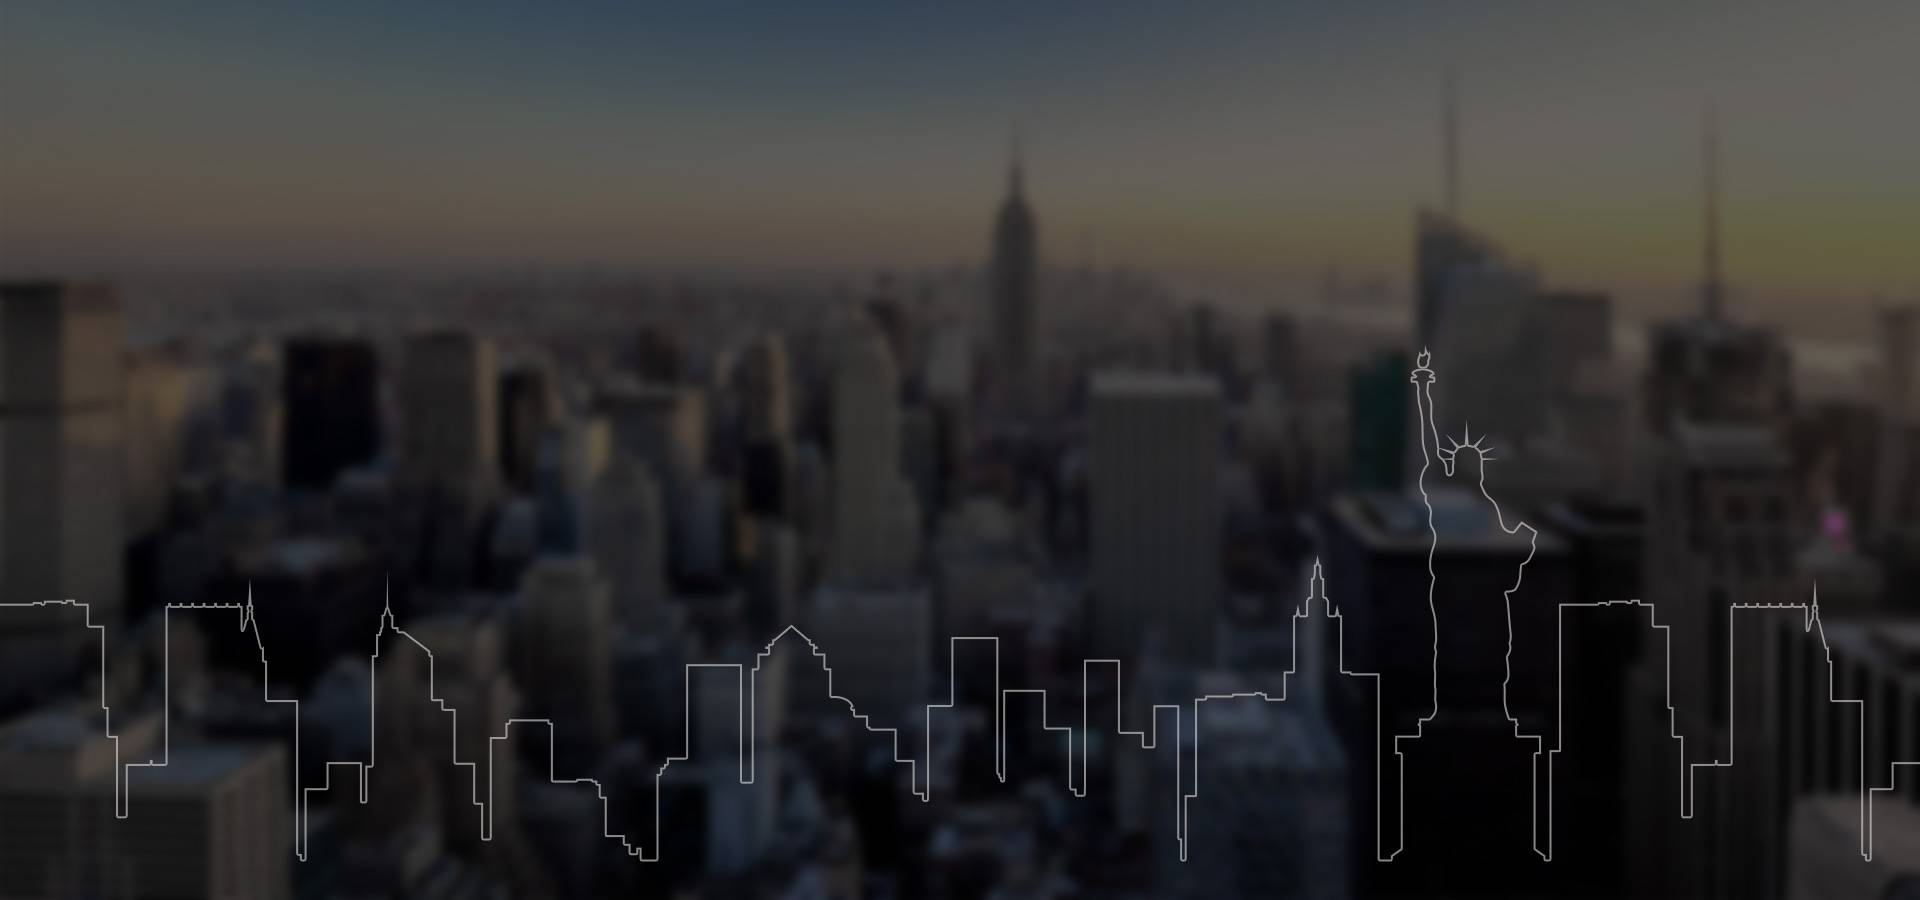
\includegraphics[width=\linewidth]{root/explorer_banner.jpg}~\\[1cm]


\includegraphics[width=0.4\textwidth]{root/oticon.png}~\\[1cm]

\vspace{2cm}


\textsc{\Large Oticon Audio Explorers challenge 2023}\\[0.5cm] % Minor heading such as course title

% Title
\hrule
\vspace{.5cm}
\centering
{ \Large \textbf{Sound Scene Classifier for Hearing Aids }}\\% title of the report
\vspace{.5cm}

\hrule
\vspace{1.5cm}


\textsc{\textbf{Team Bihotz}}\\
\begin{table}[H]
\centering
\label{tab:my-table}
\begin{tabular}{P{6cm}}
Aiax Faura Vilalta\\
Irene Campillo Pereda\\
\end{tabular}
\end{table}

\vspace{2cm}

\centering \today % Dags dato
\end{center}
\end{titlepage}

\newpage
\doublespacing
%\addcontentsline{toc}{section}{Table of Contents}
\renewcommand{\baselinestretch}{1}\normalsize
\tableofcontents
\renewcommand{\baselinestretch}{1}\normalsize
%\singlespacing
\thispagestyle{fancy} % force page style

\newcolumntype{P}[1]{>{\centering\arraybackslash}p{#1}}


\newpage
\pagenumbering{arabic} 
\fancyfoot[C]{Page \thepage\ of \pageref{LastPage}}



\section{Introduction}
The purpose of this project was designing a sound environment classifier using supervised learning techniques. The objective of this classifier is to automatically detect the nature of the sound environment to be able to adjust the settings of a hearing aid accordingly. 


\section{Data}
The training dataset consisted of 52890 sound samples, each containing 32 frequency bands, of which each has 96 time frames.
It was labeled with five different classes of sound environments with the data distribution from Figure \ref{fig:Data_distribution}.
\begin{figure}[H]
	\centering
	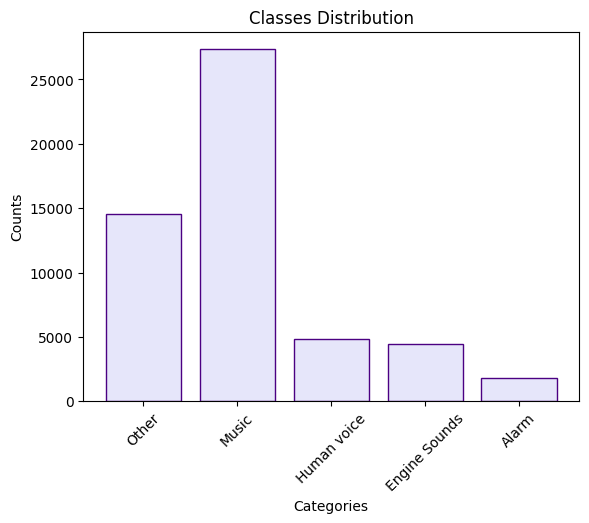
\includegraphics[width=12cm]{figures/data_distribution.png}
	\caption{Training set distribution}
	 \label{fig:Data_distribution}
\end{figure}
 The data was already preprocessed using the mel-scale, so no further preprocessing was necessary. 
 
\section{Evaluation}
Before implementing the model is important to define the evaluation methods to see how the model performs for this specific problem. After considering different methods, the following were considerate appropriate for this case.
\subsection{Accuracy}
Accuracy is perhaps the simplest metric one can imagine and is the proportion of sound scenes predictions the model got right.
However, this metric can sometimes be misleading because high accuracy does not always mean good results. For example, for this data distribution, Music and Other account for 80\% of the total data. So if the model predicted the data belonging to this classes correctly and the other ones wrong, would still get 80\% accuracy which can be considered good. However, the other three classes are more critical. As stated in the challenge, it is important for the hearing-impaired listener to hear a vehicle approaching from behind in order navigate safely. And usually, the emergency of an alarm or the conversation coming from human voice will have priority over hearing music. Is because of this that the confusion matrix is considered a better evaluation for this project.
\subsection{Confusion matrix}
A confusion matrix shows the true positive, false positive, true negative, and false negative predictions made by the model. It helps to identify which classes the model is performing well on and which ones it is struggling with. To get a fast sense on how the model is performing for each category let's look at the F1-score.
\subsection{F1-score}
Precision measures the proportion of correctly predicted instances for a particular class, out of all instances that were predicted to belong to that class. While recall measures the proportion of correctly predicted instances for a particular class, out of all instances that actually belong to that class. For example, let's say there's 300 audio clips that belong to the class "alarm": 
\begin{itemize}
  \item Precision for "alarm": The classifier predicted that 50 audio clips are "alarm", but only 40 of them are actually "alarm". The remaining 10 are false positives. Therefore, the precision for "alarm" is 40/50 = 0.8.
  \item Recall for "alarm": Out of the 300 audio clips that are actually "alarm", the classifier correctly predicted 40 of them. The remaining 260 are false negatives. Therefore, the recall for "alarm" is 40/300 = 0.133.
\end{itemize}
Since for this case it is important both to trust that what the predictions say is true (precision), and that no audios are left out of the class predictions (recall), both metrics are useful. And F1-score combines recall and precision, so it can be estimated how the model performs for each class by looking at this.


\section{Model}
 The neural network architecture that we defined for the sound environment classifier was designed to be computationally efficient and have a low memory footprint, while still being able to achieve high accuracy in classifying sound environments.
\\
\\
We chose a convolutional neural network (CNN) architecture because they are well suited for processing 2D inputs such as images and spectrograms. Convolutional layers can learn features at different scales by applying filters of different sizes to the input, and max pooling layers can reduce the spatial dimensionality of the feature maps while retaining the most important information.



\subsection{Architecture}
The architecture that we defined has two convolutional layers with relatively small filter sizes (3x3) and moderate numbers of filters (16 and 32). See figure  \ref{fig:Model architecture}. The small filter size allows the network to learn local features, while the moderate number of filters ensures that the network can learn more complex features without overfitting. The use of max pooling layers after each convolutional layer reduces the spatial dimensionality of the feature maps and helps to prevent overfitting.
\\
\\
The architecture also includes a dense layer with 64 units, which is followed by a softmax output layer with 5 units (one for each sound environment class). The dense layer allows the network to learn higher-level features that combine the local features learned by the convolutional layers.
\begin{figure}[H]
	\centering
	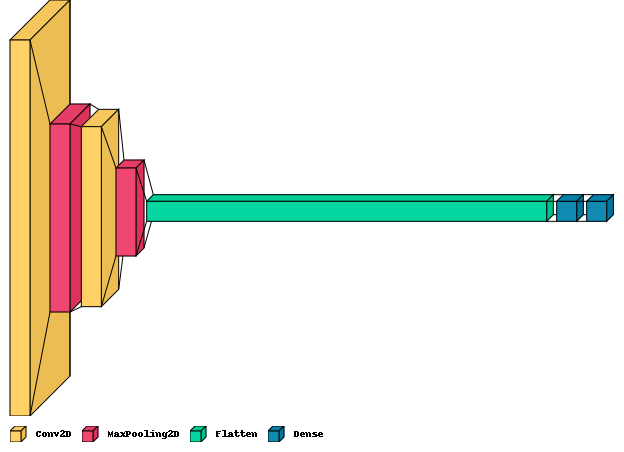
\includegraphics[width=10cm]{figures/model_architecture.png}
	\caption{Model architecture}
	 \label{fig:Model architecture}
\end{figure}
The model architecture has been defined based on the ones proposed by the papers \cite{piczak2015}, \cite{salamon2017} and \cite{politis2018}, but adapting them to strike a good balance between model complexity and computational efficiency. This architecture has a total of 275,525 parameters, almost half of the maximum recommended 500,000.
\\
\\
All the implementations made for this project as well as the model weights can be found in this Github repository
{\url{https://github.com/notaiax/Sound-scene-classifier-for-hearing-aids-ML}}



\subsection{Training, validation and test sets distribution}
Many distributions were tested to train the model. The one that gave best results was (Training set: 80\%, Validation set: 20\%). 
\\
However, the final model was trained on equally stratified data with (Training set: 80\%, Validation set: 15\%, Test set: 5\%), so the model was able to see as much as possible of the data while we could still reassure that it generalizes on data never seen before. And since it's a large dataset, 5\% is enough to validate. Even though this model peformed slightly worst than the first one, it was close enough and we can be sure that it doesn't overfit the training dataset.


\section{Results}
We see from Figure \ref{fig:Evaluation results} that the chosen model performs adequately on the validation set, as the diagonal from the confusion matrix has a stronger color, and the F1-score for all classes except from "Engine sounds" are higher than 80\%. As we can see in the confusion matrix, most of the missclassified "Engine Labels" were predicted as "Others", this could be because as stated in the challenge, "Others" can cointain sounds from different classes, "Engine Sounds" in this case. This could be solved by removing the misleading sounds from the training dataset.
\\
\\
However, for the test set (see Figure \ref{fig:Evaluation results 2}) we see that the model don't generalize well in the 3 categories with less data, which happen to be the most important. So a possible improvement would be to balance the data with data augmentation.

\begin{figure}[H]
\makebox[\textwidth][c]{
  \begin{minipage}{\textwidth}
    \centering
    \begin{minipage}{.5\textwidth}
      \centering
      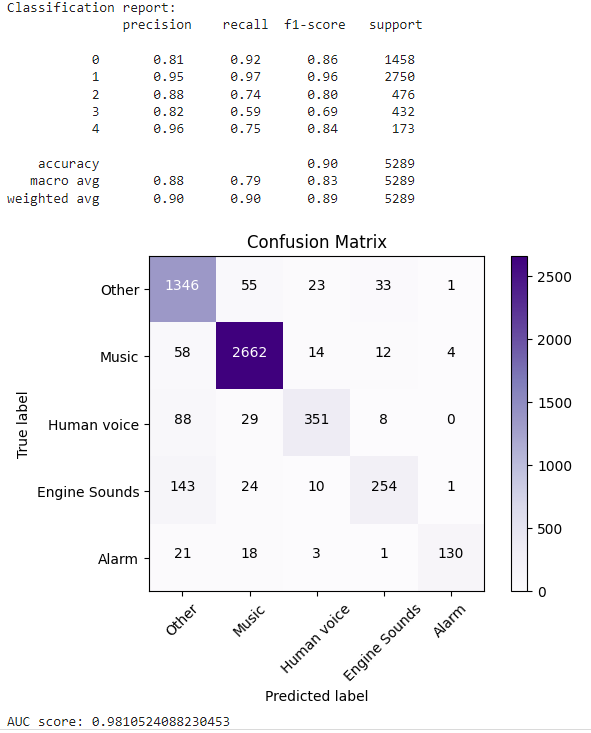
\includegraphics[width=10cm, height=12cm]{figures/Evaluation results.PNG}
      \captionof{figure}{Evaluation results on validation set}
      \label{fig:Evaluation results}
    \end{minipage}%
    \begin{minipage}{.5\textwidth}
      \centering
      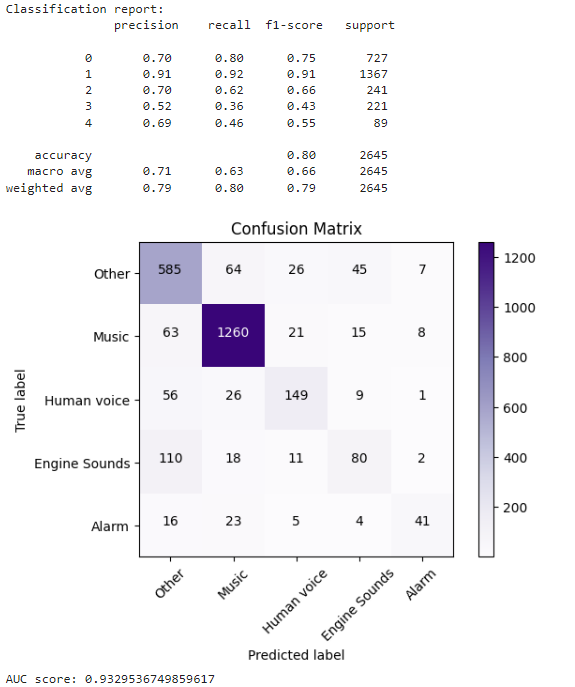
\includegraphics[width=10cm, height=12cm]{figures/Evaluation results Model 5 (on new data).png}
      \captionof{figure}{Evaluation result on test set}
      \label{fig:Evaluation results 2}
    \end{minipage}
  \end{minipage}\hspace*{0.3in}
}
\end{figure}


\section{Costs}
The prediction time for each sample is: 1.96 milliseconds. Which should be more than enough for the purpose of this project.
\\
\\
The total training time for the model on Google Colab was 17min 23s with CPU and 1min 24s with GPU. During the training, CPU models have generally performed better and the final model was trained on CPU. 


\section{Future work}
These are possible ways to improve the results that could not be tested and have been left as future work:

\begin{itemize}
  \item It may be beneficial to collect more data or use data augmentation techniques to increase the size and diversity of the dataset. \cite{towardsdatascience_audio_dl_3}
  \item The model could be improved by giving more importance and get better at detecting prioritary categories like alarms, engine sounds and human voice. This can be done with the following techniques:
  \begin{itemize}
      \item Data augmentation to balance the data and improve the performance on the most important classes because they have less data.
      \item  Class weighting to assign higher weights to the prioritary categories during training to give them more importance. This can be done by setting the class\_weight parameter in the Keras fit method. 
      \item  The thresholds for the priority classes could be lowered so they have a higher chance of being predicted. However, this case should be studied and tested deeply before being applied.
    \end{itemize}
  \item Use predictions explainability to see why the model makes the predictions it makes. This can be done with different tools such as Lime\cite{lime} and could help finding patterns in the data, see if the model predictions are reliable or just good by coincidence, and it also could help see why it missclassified "Engine Sounds" and possibly help cleaning the data.
  \item Finally, it would be important to test the model in real-world scenarios to validate its effectiveness in a hearing aid with realistic constraints on power consumption, memory, and processing power.

\end{itemize}


\section{Conclusions}
In conclusion, this project aimed to design a sound environment classifier using supervised learning techniques to automatically detect the nature of the sound environment and adjust hearing aid settings accordingly. A convolutional neural network (CNN) architecture was chosen for its ability to efficiently process 2D inputs and learn features at different scales. The model was trained on a dataset of 52,890 sound samples and achieved satisfactory results on the validation set, with most classes having an F1-score higher than 80\%, except for "Engine Sounds."
\\
However, the model's performance on the test set revealed that it did not generalize well for the three categories with less data, which are the most critical for the hearing-impaired listener. This issue could potentially be addressed by collecting more data, using data augmentation techniques, or adjusting the class weighting and thresholds during training.
\\
\\
Although is usually recommended to train CNN's on GPU, smaller CNN's sometimes perform better when trained on CPU and this was the case during this project.
\\
\\
The prediction time of 1.96 milliseconds per sound sample is deemed sufficient for the intended purpose of this project. Nonetheless, there is room for improvement, and future work may include refining the model to better detect priority categories, employing predictions explainability to understand the model's decision-making process, and testing the model in real-world scenarios to assess its effectiveness in actual hearing aid devices.
\\
\\
Overall, this project represents a promising step towards the development of intelligent hearing aids capable of adapting to different sound environments, improving the quality of life for hearing-impaired individuals.



\newpage
\begin{thebibliography}{9}

\bibitem{piczak2015}
Piczak, K. J. (2015). Environmental sound classification with convolutional neural networks. In \textit{2015 IEEE International Workshop on Machine Learning for Signal Processing, Sept. 17-20, 2015, Boston, USA}.

\bibitem{salamon2017}
Salamon, J., \& Bello, J. P. (2017). Deep Convolutional Neural Networks and Data Augmentation for Environmental Sound
Classification. In \textit{IEEE Signal Processing Letters, accepted November 2016}.

\bibitem{politis2018}
Zeinali, H., Burget, L., & Cernocky, J. (2018). Convolutional neural networks and x-vector embedding for DCASE2018 acoustic scene classification challenge. In \textit{Detection and Classification of Acoustic Scenes and Events 2018, November 19-20, 2018, Surrey, UK}.
\bibitem{github_project}
Faura Vilalta A., Campillo Pereda I.
\textit{Sound Scene Classifier for Hearing Aids},
GitHub repository,
\url{https://github.com/notaiax/Sound-scene-classifier-for-hearing-aids-ML},
2023,
Accessed: April 23, 2023.

\bibitem{towardsdatascience_audio_dl_3}
Ketan Doshi. \textit{Audio Deep Learning Made Simple - Part 3: Data Preparation and Augmentation.}
\textit{Towards Data Science}, February 24, 2021.
\url{https://towardsdatascience.com/audio-deep-learning-made-simple-part-3-data-preparation-and-augmentation-24c6e1f6b52}.

\bibitem{lime}
Marco Tulio Ribeiro, Sameer Singh, Carlos Guestrin. \emph{"Why Should I Trust You?": Explaining the Predictions of Any Classifier.\url{https://dl.acm.org/doi/10.1145/2939672.2939778}}. 2016

\end{thebibliography}

\end{document}
